%\addcontentsline{toc}{chapter}{Development Process}
\chapter{Design}

In this section I will describe my design as of the date of the project outline description. \\
This is the design I will follow and try to implement, however this is more of a guideline rather than exact plan since I have to figure out what the API and simulator are able to do and what I am able to implement inside the given time.\\

\section{Environment Design}
The final environment which I will create for this project will consist of a large starting area, with a corridor adjacent to it. The corridor will hold 1 smaller room to either side, 1 of them with an obstacle inside which will have to be traversed and mapped. The size of the corridor should not be to big so that it is still a challenge to move through it however it should rather not be to small to make movement through it too problematic. \\
A to small size could also make the corridor not distinctive enough from the rest of the wall so the E-Puck could have problem registering and moving into it.\\

\begin{figure}[h]
\centering
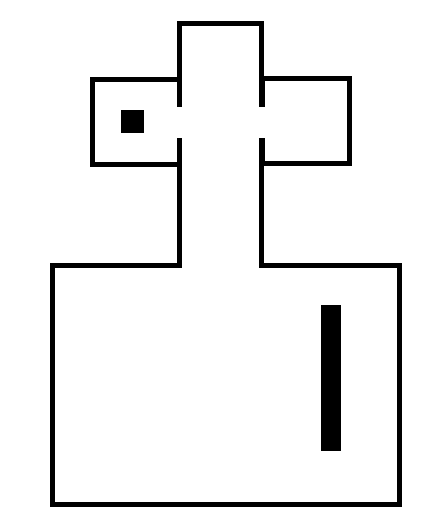
\includegraphics[width=0.5\textwidth]{../../figures/environment_example.png} 
\caption{Environment Design}
\label{Figure 2}
\end{figure}

\section{Mapping and Swarm Size}
For mapping I will use a occupancy grid, and the occupancy will be acquired by the E-Puck's laser sensors. 
I will yet have to decide on a resolution, for the grid.\\
I will use a swarm of 5 E-Puck robots, of which 1 will remain stationary and only function as the "Uplink point" to which all robot send the acquired data. 
The stationary robot will also be used as reference point for the localisation method.

\section{Deployment}
I am of this moment still undecided for which deployment strategy will be implemented. \\
There are 2 deployment strategies which I decided for based on the background research I have done.\\[3ex]

One of them is based on a nearest neighbour approach in which the robots will emit signals to each other which will cause them to drive away from each other until a previous maximum communication distance has been reached. This relationship between robots could be described similar to magnets which can repulse and pull in each other in order to hold a given maximum distance and thereby cover the largest possible area\\
The movement of the robots would be a random walk with included obstacle avoidance. One possibility could be to add a wall following functionality to it as well. However this would require some form of higher functions which to keep the robot from being stuck inside a loop. These higher functions could work by keeping track of the robots position on the map and react once the robot starts traversing the same area again, in this case the algorithm could force to robot back into a random walk.\\[3ex]

The other deployment strategy would implement a more controlled movement pattern. This pattern would move the robots inside a rectangular pattern which would implement a function to move around obstacles on the way before moving back into the original pattern. 
While this reason is more controlled I am not sure which one will turn out to be more effective, that it why I will implement both inside a testing phase and will then decide which of them I will use.